\documentclass[utf8, diplomski]{fer}
%\documentclass[utf8, diplomski, upload]{fer}
\usepackage{booktabs}
\usepackage{indentfirst}
\usepackage{subcaption}
\usepackage{placeins}
\usepackage{float}
\usepackage{cite} % Za bibliografiju
\usepackage{url} % Za web adrese
\usepackage{listings}
\usepackage{caption}
\usepackage{tabularx}

\usepackage{mathptmx} % Use Times New Roman font
\usepackage{setspace} % For setting line spacing
\onehalfspacing % Set line spacing to 1.5

\captionsetup[lstlisting]{labelfont=bf,labelsep=period,font=small}

% Tvoj postojeći kod ostaje isti
\lstset{
    basicstyle=\ttfamily\small,
    breaklines=true,
    frame=single,
    backgroundcolor=\color{gray!5},
    keywordstyle=\color{blue},
    commentstyle=\color{green!50!black},
    stringstyle=\color{orange},
    captionpos=b,
    lineskip=-1.5pt
}

\renewcommand{\lstlistingname}{Kod}

\AtBeginDocument{
    \renewcommand{\thelstlisting}{\arabic{chapter}.\arabic{lstlisting}}
}

% 2. Dodatak za hyperref kako bi \autoref{...} ispisivao "Kod X.Y" umjesto samo broja
\newcommand{\lstlistingautorefname}{Kod}


\usepackage{titlesec} % To control the title spacing
\titlespacing*{\chapter}{0pt}{-50pt}{20pt}

\renewcommand{\figurename}{Slika}
\renewcommand{\bibname}{Literatura}
\renewcommand{\tablename}{Tablica}
\renewcommand{\contentsname}{Sadržaj}
\renewcommand\thepage{}

\title{Implementation of a centralized system for monitoring and visualizing local network communication patterns}
\naslov{Implementacija središnjeg sustava za nadzor i vizualizaciju komunikacijskih obrazaca lokalne mreže}
\brojrada{1586}
\author{Ante Čavar}
\datum{lipanj, 2026.}
\mentor{prof.dr.sc. Stjepan Groš}

\begin{document}
\maketitle
\zadatak{hr_0036540817_94.pdf}
\begin{zahvale}
Zahvaljujem svojoj obitelji što je uvijek bila uz mene.
\end{zahvale}
\newpage
\tableofcontents
\newpage
\mainmatter
\setcounter{page}{1}
\renewcommand\thepage{\arabic{page}}
\chapter{Uvod}

Svaki uređaj danas je povezan u neku mrežu. Velika većina tih uređaja pripada jednoj od bezbroj lokalnih mreža. Neke su kućne, neke poslovne, a neke vojne.
Činjenica je da su lokalne mreže svugdje oko nas. Sigurnost lokalnih mreža (kao i sigurnost bilo čega drugog) nije pratila razvoj i pristupačnost tih istih mreža.
Jednom kada se sigurnosni incidenti krenu nizati se krene buditi i svijest poslovnih i privatnih korisnika.

Kako bi se incidenti (a time i troškovi pogotovo za poslovne korisnike) izbjegli na tržištu se pojavilo mnoštvo programa\cite{splunk_docs}\cite{security_onion} pa čak i zanimanja (SOC analist).
Ta rješenja funkcioniraju za one koji ih mogu platiti. Ako postoji potreba za pravim 24 satnim nadzorom onda firmi nije problem zaposliti (najmanje) 3 SOC analista koji će se izmjenjivati u 8 satnim
smjenama. Postoji i mogućnost računalne zaštite koja nije toliko dobra ali i dalje nudi neku razinu zaštite. No ipak problem svih navedenih rješenja je što koštaju.

Cilj ovog rada je ponuditi programsko rješenje osobnim korisnicima i malim firmama kako bi zaštitili svoju lokalnu mrežu unatoč manjoj financijskoj sposobnosti koja nije problem za veće firme zbog toga što su male firme cilj
nemalog broja napada čak 43\%\cite{totalassure_smallbusiness}.
U radu su obrađena dva moguća rješenja gore navedenog problema. Korišteni alati sa kojima se radilo je Zeeku kao osnovnom alatu za prikupljanje podataka, nakon toga se ispitivanje provodilo nad 2 para 
baze podataka i njezinim agregatorom podataka: InfluxDB uz Telegraf kao agentu za prikupljanje podataka te Elasticsearch uz Filebeat Obje baze podataka na kraju su informacije agregirale u Grafani za vizualizaciju 
prikupljenih informacija.

Nakon objašnjenja rada i procesa ponuditi će se čitateljima mogući smjerovi za ovo implementacijsko rješenje te koje daljnje korake autor vidi u ovom radu.
\chapter{Teorijska podloga i tehnološki stog}
NSM (eng. \textit{Network Security Monitoring}) predstavlja metodologiju prikupljanja, analize i eskalacije indikatora koji ukazuju na maliciozne aktivnosti unutar nekog mrežnog okruženja. 
Tradicionalni mehanizmi zaštite kao vatrozid i antivirusi se primarno fokusiraju na prevenciju napada izgradnjom barijera. Međutim, kako ističe 
Bejtlich \cite{bejtlich_nsm}, prevencija s vremenom zakazuje, a napadači kontinuirano pronalaze nove načine za zaobilaženje statičkih obrana.
Zato se NSM ne oslanja isključivo na prevenciju nego i na dubinsku vidljivost mrežnog prometa koja omogućava pravovremenu detekciju i reakciju na incidente.

Kako bi se uspostavio funkcionalan NSM sustav, potrebno je integrirati nekoliko različitih klasa alata: od mrežnih senzora za ekstrakciju metapodataka, preko optimiziranih baza podataka za 
pohranu vremenskih nizova, do grafičkih sučelja za vizualizaciju anomalija. 
U nastavku ovog poglavlja bit će opisane teorijske osnove tehnologija koje su odabrane kao temelj za izgradnju takvog rješenja.

\section{Mrežna infrastruktura i pristupne točke}
AP (eng. \textit{Access Point}) još znan i kao pristupna točka je uređaj koji se ponaša kao most (eng. \textit{bridge}) i time dopušta bežičnim uređajima poput laptopa, mobitela, IoT senzora 
da se povežu sa žičanom lokalnom mrežom (LAN). Za razliku od bežičnih rutera koji u sebi kombiniraju preusmjeravanje, vatrozid i WiFi funkcionalnosti pristupne točke se fokusiraju u potpunosti 
na bežično povezivanja (iako se danas ta granice između pristupne točke i rutera sve manje primjećuje).

\texttt{hostapd} je alat na Linuxu s kojim se može jedan od bežičnih mrežnih sučelja sustava pretvoriti u pristupnu točku \cite{hostapd_docs} pod uvjetom da postoji još jedno mrežno sučelje (žičano ili mrežno) 
koje će služiti kao izlaz na Internet. Između ostalog \texttt{hostapd} nudi mogućnosti:
\begin{itemize}
    \item nadzora pristupne točke preko IEEE 802.11 standarda
    \item autentifikacijske protokole poput IEEE 802.1X, WPA, WPA2, i WPA3
    \item može funkcionirati kao RADIUS Server/Klijent što je posebno bitno firmama i ustanovama
\end{itemize}

Kako bi uređaji povezani na pristupnu točku mogli funkcionalno komunicirati, potrebno je osigurati mrežnu konfiguraciju i razlučivanje naziva. Ulogu pružanja tih servisa u sustavima s ograničenim 
resursima često preuzima alat \texttt{dnsmasq} \cite{dnsmasq_docs}. Potrebno je naglasiti da \texttt{dnsmasq} ne obavlja izolaciju ili usmjeravanje mrežnog prometa (što je primarni zadatak vatrozida), 
već isključivo objedinjuje funkcionalnosti DNS prosljeđivača (eng. \textit{DNS forwarder}) i DHCP poslužitelja.

U ulozi DNS prosljeđivača, \lstinline|dnsmasq| prihvaća lokalne DNS upite te ih prosljeđuje vanjskim DNS poslužiteljima kako bi se simbolička imena (domene) prevela u odgovarajuće IP adrese. Kao DHCP 
poslužitelj (eng. \textit{Dynamic Host Configuration Protocol}), zadužen je za automatsku dodjelu mrežnih parametara. DHCP poslužitelj se brine da se svakom uređaju koji pristupa mreži dinamički dodijeli 
jedinstvena IP adresa, podmrežna maska i adresa zadanog usmjernika, čime se omogućava neometana komunikacija i izbjegavaju mrežne kolizije.

\section{Sustavi za detekciju upada i analizu prometa}
Zeek je platforma otvorenog koda namijenjena dubinskoj analizi mrežnog prometa. Za razliku od tradicionalnih sustava koji se oslanjaju na bilježenje sirovih mrežnih paketa, Zeek generira 
kompaktne transakcijske zapisnike (eng. \textit{transaction logs}) visoke preciznosti te omogućava potpuno prilagodljiv izlazni format podataka. Time se analitičarima osiguravaju konkretni i primjenjivi 
podaci (eng. \textit{actionable data}). Neovisno o veličini okruženja -- od malih lokalnih mreža do opsežnih istraživačkih i komercijalnih sustava -- Zeek pruža jasan uvid u obrasce korištenja mreže, 
čime izravno doprinosi nadzoru sigurnosti, reviziji i analizi mrežnih performansi.

Jedna od ključnih prednosti ovog sustava je njegov specifičan, mrežno optimiziran skriptni jezik koji omogućava izradu prilagođenih pravila detekcije i ekstrakciju specifičnih metapodataka. Zahvaljujući 
globalnoj prihvaćenosti i snažnoj podršci zajednice otvorenog koda, Zeek nudi dubinske uvide neophodne za rješavanje najsloženijih sigurnosnih izazova unutar poslovnih, računalnih i \textit{cloud} 
okruženja.

Najveća prednost Zeeka je mogućnost kreiranja logova ovisno o tipu povezivanja i protokola (\texttt{conn.log, dhcp.log, http.log, files.log, dns.log ...}). Osim podjele na protokole Zeek nudi i jedinstvenu 
mogućnost upozorenja (\texttt{notice.log}) gdje se korištenjem Zeekovog skriptnog jezika mogu prepoznati specifični tipovi povezivanja ili se uočiti obrasci u ponašanju uređaja u mreži.

Alternative poput Suricata fokusiraju se primarno na detekciju temeljenu na potpisima (eng. \textit{signature-based detection}). Sveobuhvatna rješenja poput 
Security Oniona, iako funkcionalna, zahtijevaju znatno veće resurse — minimalno 12\,GB RAM-a za osnovnu instalaciju \cite{security_onion}\cite{security_onion_hwreq} — što ih čini 
neprikladnima za deployment na potrošačkom hardveru. Zeekova prednost leži u fleksibilnoj ekstrakciji metapodataka i prilagodljivom skriptnom jeziku koji 
omogućava izradu vlastite detekcijske logike uz minimalni memorijski otisak.

\section{Kontejnerizacija mrežnih servisa}
Docker je platforma za razvoj, dijeljenje i pokretanje aplikacija. Omogućava odvajanje aplikacija od infrastrukture \cite{docker_docs}. Kako bi to efikasno napravio, Docker koristi kontejnere.

Kontejneri su mala okruženja koja se pokreću na računalu domaćinu te su izolirana od ostalih procesa korištenjem \textit{namespaceova} i \textit{cgroups} tj. kontrolnih grupa. Kontejneri su 
pokretljive instance slika (eng. \textit{images}) koje možete izraditi, pokrenuti, zaustaviti, premjestiti ili izbrisati pomoću Docker alata. Također su portabilni te se mogu pokrenuti lokalno,
u virutalnim strojevima i u oblaku. 

Docker se pobrinuo da kontejneri imaju minimalan utjecaj na domaćina te za pokretanje kontejnera nije potrebna instalacija dodatnih ovisnosti na sustavu domaćina. Svaki se kontejner pokreće u 
izoliranom okruženju te može komunicirati sa ostalim kontejnerima tek ako mu se to eksplicitno dozvoli.

Za orkestraciju više kontejnera koji zajedno čine jednu aplikaciju Docker nudi alat Docker Compose. Konfiguracija cijelog skupa servisa definira se u jednoj 
\textit{docker-compose.yml} datoteci koja opisuje svaki servis, njegove ovisnosti, volumene i mrežne postavke. Pokretanje cijelog sustava svodi se na jednu naredbu 
(\lstinline|docker compose up -d|), što znatno pojednostavljuje deployment i reproducibilnost okruženja te je glavni razlog zašto je upravo Docker korišten u ovom radu.

\section{Pohrana vremenskih nizova i vizualizacija}
InfluxDB je baza podataka temeljena na Time-Series modelu te koristi Flux jezik za upite. Time-series model baze je optimiziran da sprema, indeksira i izvršava upite nad podatcima gdje je vrijeme 
glavna organizacijska dimenzija.\cite{influxdb_docs} Glavne karakteristike InfluxDB baze podataka: \begin{itemize}
    \item indeksiranje temeljeno na vremenu (omogućava brzu obradu velikih količina podatka)
    \item samo "nadodaj" (eng. \textit{append}) arhitektura (nijedan se zapis ne briše ili uređuje što omogućava pristup povijesti izmjena)
    \item optimizirano sažimanje i pohrana (koristi kompresiju na temelju vremena te tehnike smanjenja uzorkovanja da lakše rukuje velikim volumenom podataka)
    \item ugrađene agregacijske funkcije (podrška za vremenski specifične funkcije poput pomičnih prosjeka, percentila i sažetaka temeljenih na intervalima olakšava složenu analizu bez velikih računalnih troškova)
\end{itemize}
InfluxDB podržava tri moguća jezika upita: SQL, Flux i Influx. U ovom radu korišten je Flux zbog odabrane verzije baze (2.7). Flux je funkcionalni skriptni jezik otvorenog koda dizajniran za upite, 
analizu i djelovanje na podacima vremenskih serija, prvenstveno služeći kao izvorni jezik upita za InfluxDB 2.x.\cite{flux_getstarted}\cite{flux_basics_video} Za razliku od SQL-sličnog InfluxQL-a koji se koristi u InfluxDB 1.x, 
Flux je dizajniran da bude kompozibilan i fleksibilan, podržavajući ne samo InfluxDB već i razne SQL baze podataka (npr. PostgreSQL, BigQuery) i formate podataka poput CSV-a i JSON-a.
Primjer Flux upita: \cite{flux_query_basics}
\newpage
\begin{lstlisting}[language=, caption={Primjer Flux upita}, label={lst:basic_flux_query}]
import "influxdata/influxdb/v1"

option v = {bucket: "my-bucket", org: "my-org"}

from(bucket: v.bucket)
    |> range(start: -1h)
    |> filter(fn: (r) => r._measurement == "cpu")
    |> mean()
\end{lstlisting}
Upit \ref{lst:basic_flux_query} definira "kantu" informacija te se iz tog \textit{bucketa} redom povlače informacije na sljedeći način: svi logovi iz prethodnih sat vremena (\lstinline|start: -1h|),
koji u sebi sadrže informaciju o CPU-u (\lstinline|filter(fn: (r) => r._measurement == "cpu"|)) te iz tih informacija izvuci srednju vrijednost (\lstinline|mean()|). Drugim riječima ovaj upit će
prikupiti informacije o CPU-u u zadnjih sat vremena te će prikazati njihovu srednju vrijednost.

Telegraf je alat za prikupljanje podataka otvorenog koda koji je razvio InfluxData, a koji prikuplja, obrađuje i agregira metrike, logove i druge podatke iz različitih izvora. 
Služi kao primarni sloj za unos podataka za InfluxDB, bazu podataka vremenskih serija, koristeći arhitekturu temeljenu na dodacima s preko 300 ulaznih i izlaznih dodataka za prikupljanje 
podataka iz sustava, senzora i aplikacija te njihov izravan zapis u InfluxDB.\cite{telegraf_docs}\cite{influxdb_telegraf_intro}
Neke od karakteristika Telegrafa su:
\begin{itemize}
    \item Arhitektura temeljena na dodatcima (\textit{pluginovi}) (korisnik konfigurira ulaze i izlaze u \lstinline|telegraf.conf| što omogućuje fleksibilno upravljanje tokom podataka bez konkretnog znanja programiranja)
    \item Napisan u jeziku GO (jedna binarna datoteka sa mogućnošću obrade ogromne količine podataka sa više uređaja)
    \item predprocesiranje podatka (može očistiti, filtrirati i transformirati podatke prije nego što stignu do baze podataka)
\end{itemize}

Uz InfluxDB i Telegraf, kao alternativa ispitan je i Elasticsearch uz Filebeat kao agentom za prikupljanje podataka.

Elasticsearch je distribuirani sustav za pretraživanje i analizu podataka otvorenog koda temeljen na Apache Lucene biblioteci.\cite{elasticsearch_docs} Za razliku od 
InfluxDB-a koji optimizira pohranu vremenskih serija, Elasticsearch tretira svaki zapis kao JSON dokument koji se indeksira kroz invertirani indeks (eng. 
\textit{inverted index}) — struktura podataka koja omogućava brzu pretragu po sadržaju polja. Ta arhitektura čini Elasticsearch pogodnim za \textit{full-text} 
pretraživanje i korelaciju podataka iz heterogenih izvora, no dolazi s većim memorijskim i prostornim otiskom u usporedbi s InfluxDB-om što će biti detaljnije 
prikazano u poglavlju evaluacije.

Kao što Telegraf služi kao agent za unos podataka u InfluxDB, Filebeat preuzima analognu ulogu u Elasticsearch ekosustavu.\cite{filebeat_docs} Filebeat je lagani 
agent koji prati zadane datoteke zapisnika i prosljeđuje nove zapise u Elasticsearch. U kontekstu ovog rada, Filebeat čita Zeekove JSON logove iz dijeljenog volumena i 
indeksira ih u Elasticsearch bez transformacije podataka.

Grafana je platforma otvorenog koda za vizualizaciju i analizu podataka koja podržava više od pedeset izvora podataka, uključujući InfluxDB i 
Elasticsearch.\cite{grafana_docs} Dashboardi se konfiguriraju kroz grafičko sučelje i mogu se izvesti kao JSON datoteke te pohraniti u repozitorij, što 
omogućava automatsko učitavanje pri pokretanju sustava (eng. \textit{provisioning}). U ovom radu Grafana služi kao jedinstveno vizualizacijsko sučelje za oba ispitana 
backend rješenja.
\chapter{poglavlje}{Arhitektura}
U ovom se poglavlju opisuje arhitektura predloženog (kasnije i implementiranog) sustava. Opisuje se način na koji je lokalna mreža usmjerena
kroz pristupnu točku, gdje se i kako prikuplja mrežni promet te kako se prikupljeni podatci pohranjuju, vizualiziraju te u konačnici kako se s tim podatcima 
rukuje kako bi se postigla automatska detekcija. Naglasak je na odlukama o dizajnu i njihovim opravdanjima, dok se konkretna implementacija obrađuje kasnije.

\section{Pregled sustava}
Sustav je zamišljen da pretvori uređaj s mrežnim mogućnostima u jedinstvenu točku kroz koju prolazi sav promet lokalne
mreže, čime se ostvaruje potpuna vidljivost komunikacije između lokalnih uređaja i vanjskih odredišta. Taj uređaj
istovremeno obavlja funkciju usmjernika (eng.\ \emph{gateway}), pristupne točke, mrežnog senzora i vatrozida.

Slika \ref{fig:tok-podataka} prikazuje tok podataka kroz sustav. Sav mrežni promet prolazi kroz pristupnu točku gdje ga Zeek pasivno analizira i pohranjuje 
u obliku strukturiranih JSON zapisa u dijeljeni direktorij.
Iz tog se direktorija podatci paralelno "šalju" u dva odvojena podsustava za pohranu. Prvi sustav čine vremenski orijentirana baza InfluxDB posredstvom 
podatkovnog agregatora Telegrafa. Drugi sustav čine dokumentno orijentiranu bazu Elasticsearch posredstvom agenta zvanog Filebeat. 
Oba podsustava kao zajedničko vizualizacijsko sučelje koriste Grafanu. Usporedno postojanje dvaju podsustava ne predstavlja produkcijsku konfiguraciju, već
služi za njihovu usporedbu opisanu u kasnijim poglavljima. U stvarnoj bi se primjeni odabrao jedan od njih ovisno o potrebama i mogućnostima.

\begin{figure}[ht]
  \centering
  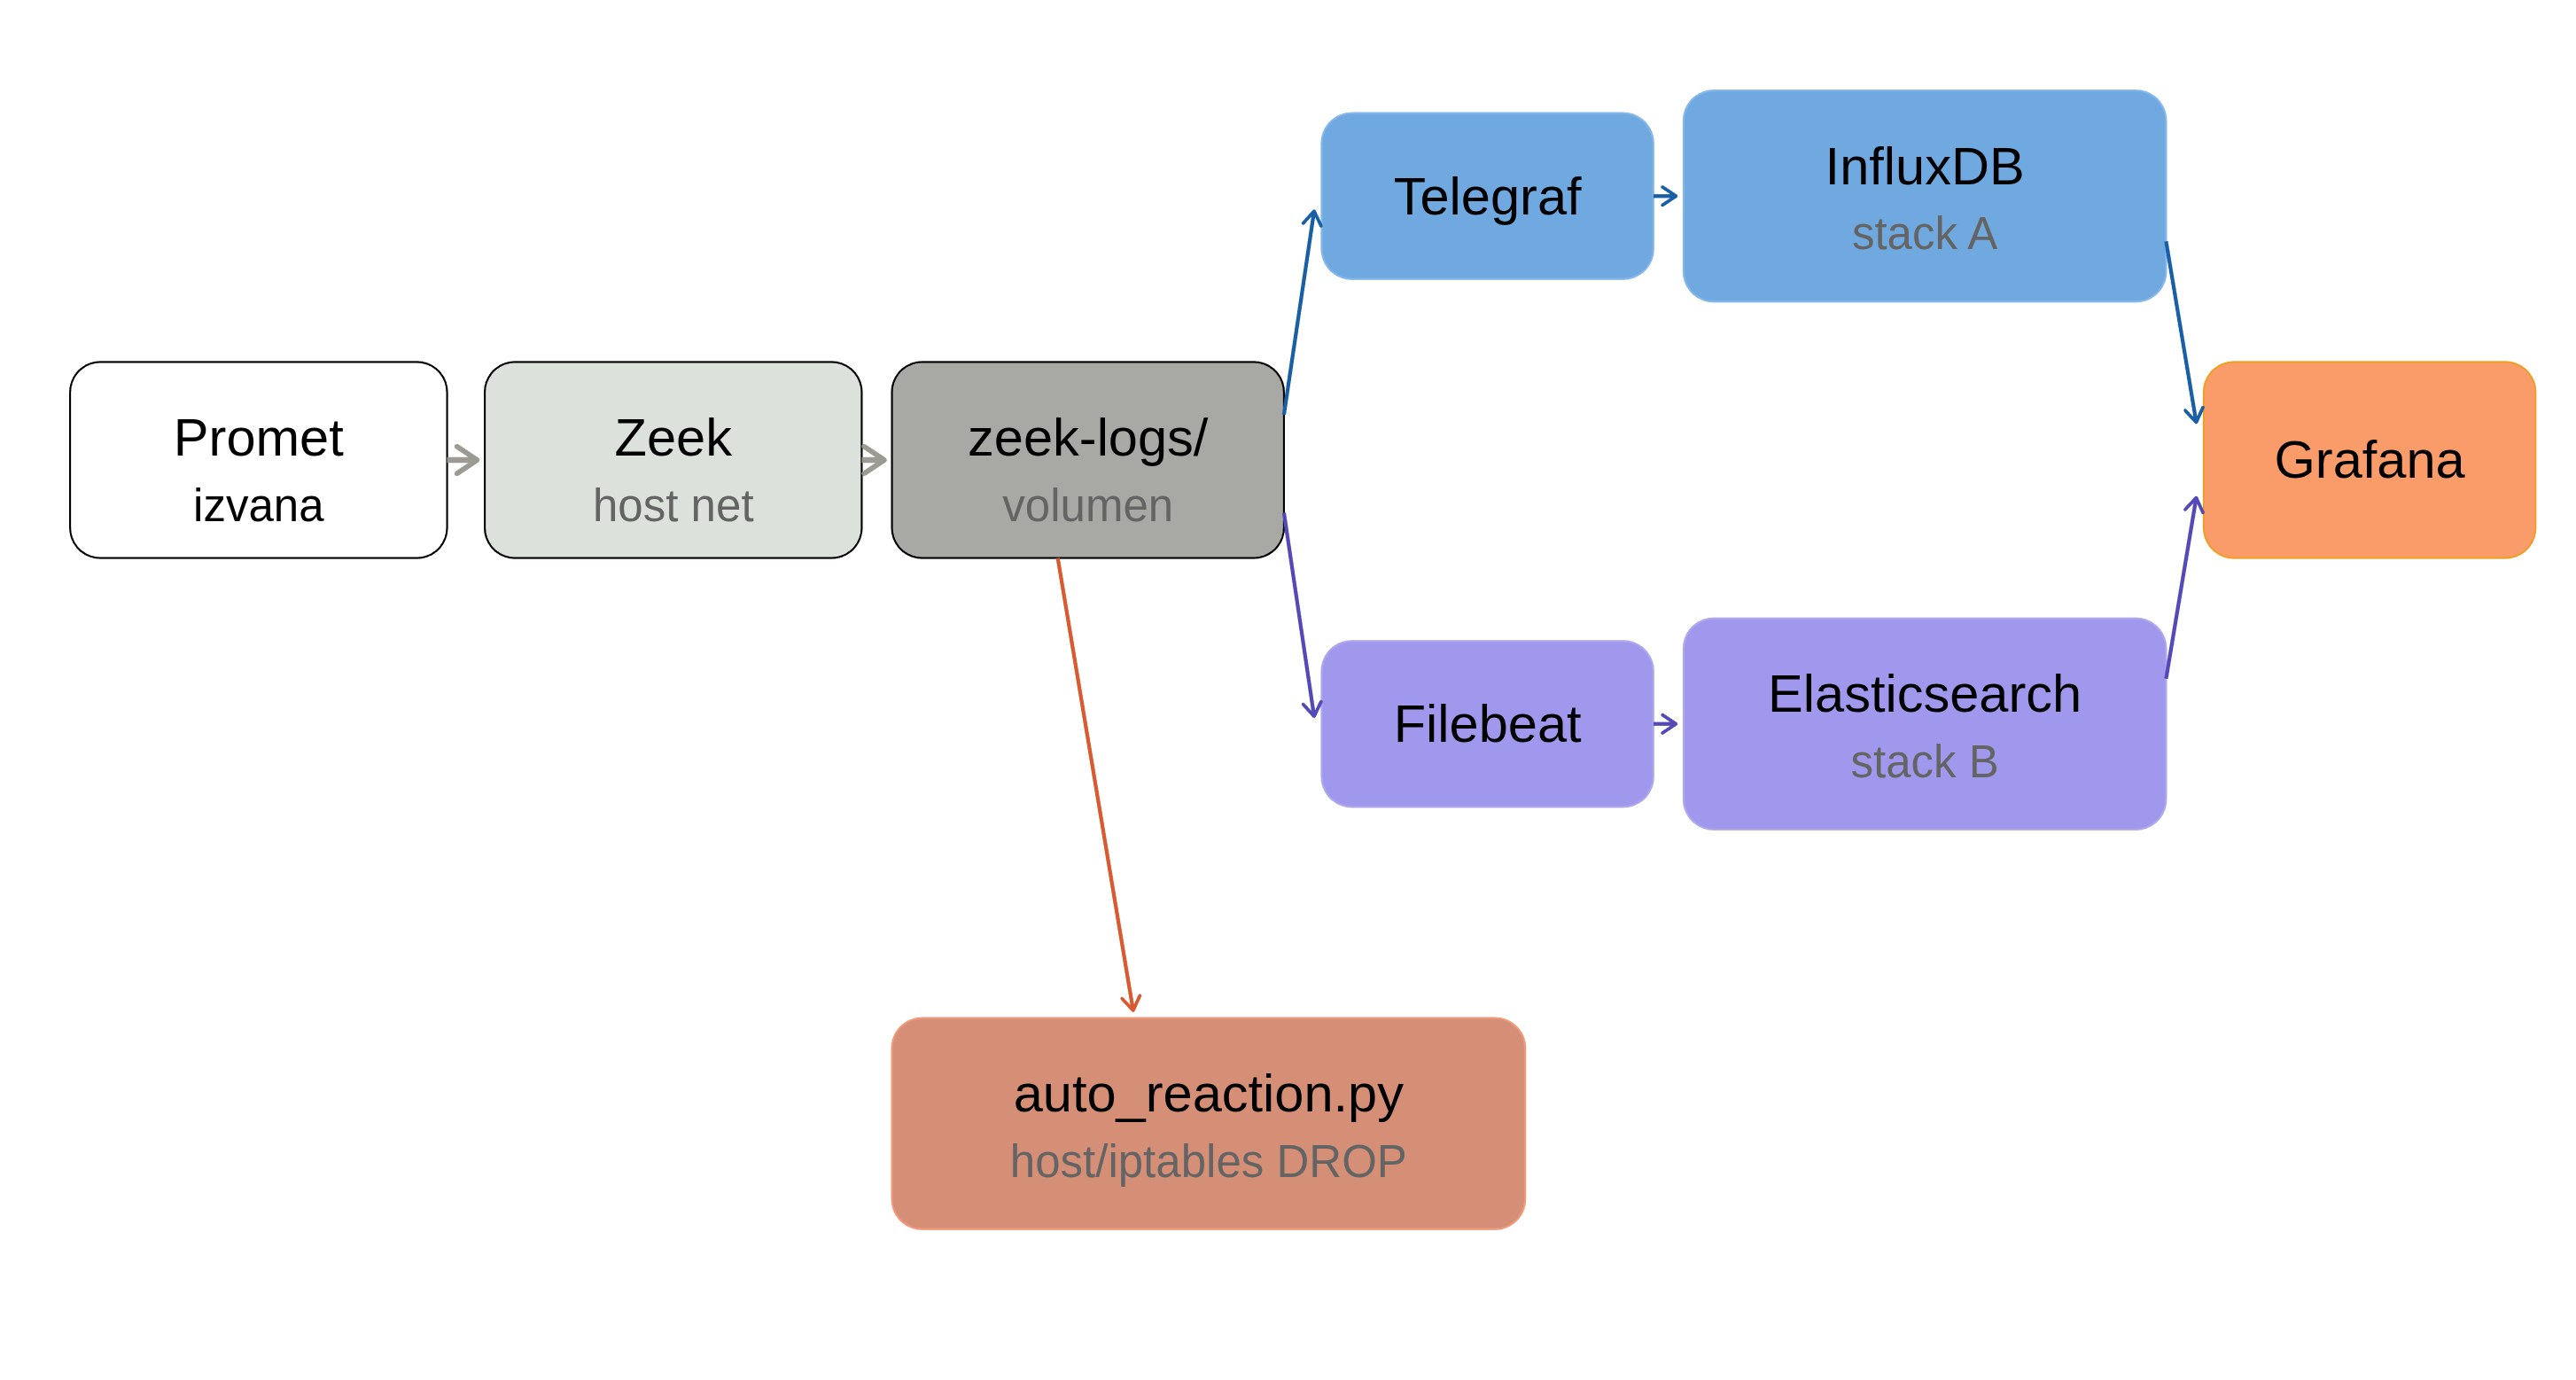
\includegraphics[width=0.95\textwidth]{slike/tok_podataka_dual_stack_custom.png}
  \caption{Prikaz toka podataka kroz sustav}
  \label{fig:tok-podataka}
\end{figure}

Svi navedeni servisi izvode se u Docker kontejnerima, čime se postiže ponovljivost i prenosivost okruženja te jednostavnost pri postavljanju \cite{docker_docs}. 
Jedina je iznimka skripta za automatsku reakciju, koja se izvodi izravno na domaćinu iz kasnije objašnjenih razloga.

\section{Mrežni sloj}
Mrežna topologija sustava prikazana je na slici \ref{fig:topologija}. 

\begin{figure}[h]
  \centering
  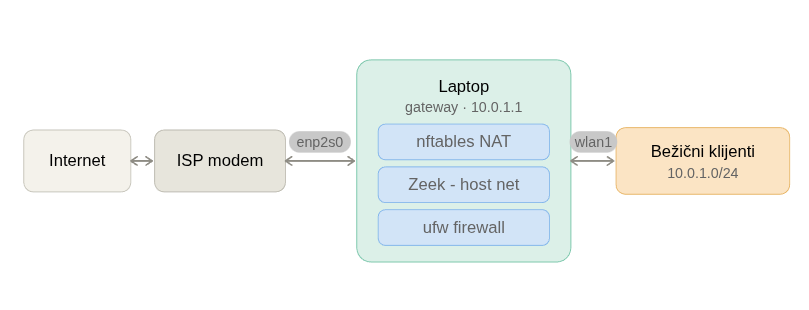
\includegraphics[width=0.95\textwidth]{slike/mrezna_topologija_custom.png}
  \caption{Mrežna topologija. Prijenosno računalo objedinjuje uloge rutera,
           pristupne točke, senzora i vatrozida}
  \label{fig:topologija}
\end{figure}

\section{Nadzorni sloj}

\section{Tok podataka i pohrana}

\section{Prepoznavanje i automatska reakcija}

\include{implementacija}
\include{evaluacija}
\include{testiranje}
\include{zakljucak}
\bibliography{literatura}


\begin{sazetak}
  None
\end{sazetak}
\begin{kljucnerijeci}
  None
\end{kljucnerijeci}
\begin{abstract}
  None
\end{abstract}
\begin{keywords}
    None
\end{keywords}

\newpage
\chapter*{Skraćenice}
\addcontentsline{toc}{chapter}{Skraćenice}
\renewcommand{\arraystretch}{2} % Increase the row spacing by 1.5 times
\begin{tabularx}{\textwidth}{>{\bfseries}p{0.15\textwidth} >{\itshape}p{0.45\textwidth} p{0.4\textwidth}}
\end{tabularx}

\end{document}

%
% % Primjer slike
% \begin{figure}[h]
%   \centering
%   \includegraphics[width=0.8\textwidth]{example-image-a}
%   \caption{Primjer slike.}
%   \label{fig:example-image}
% \end{figure}

% % Primjer tablice
% \begin{table}[h]
%   \centering
%   \begin{tabular}{|c|c|c|}
%       \hline
%       Zaglavlje 1 & Zaglavlje 2 & Zaglavlje 3 \\
%       \hline
%       Podatak 1 & Podatak 2 & Podatak 3 \\
%       Podatak 4 & Podatak 5 & Podatak 6 \\
%       \hline
%   \end{tabular}
%   \caption{Primjer tablice.}
%   \label{tab:example-table}
% \end{table}
%
% Primjer ubacivanja koda
% \begin{lstlisting}[language=Python, caption={Petlja za čitanje notice.log datoteke u stvarnom vremenu.}, label={lst:auto-reaction-petlja}]
% def process_log():
%    print(f"[*] Nadzor pokrenut nad {LOG_FILE}")
%    while not os.path.exists(LOG_FILE):
%        time.sleep(1)

%    with open(LOG_FILE, 'r') as f:
%        f.seek(0, os.SEEK_END)
%        while True:
%            line = f.readline()
%            if not line:
%                time.sleep(0.2)
%                continue
% \caption{Naslov}
% \label{lst:primjer-koda}
% \end{lstlisting}